\documentclass[stu,12pt,floatsintext]{apa7}
\usepackage[american]{babel}
\usepackage{csquotes}
\usepackage[style=apa,sortcites=true,sorting=nyt,backend=biber]{biblatex}
\DeclareLanguageMapping{american}{american-apa}
\usepackage[T1]{fontenc}
\usepackage{mathptmx}
\usepackage{graphicx}
\usepackage{array}
\usepackage{multirow}
\usepackage[labelsep=newline,labelfont=bf]{caption}
\usepackage{multicol}
\usepackage{makecell}
\usepackage{amsmath}
\usepackage{float}
\usepackage{setspace}
\usepackage{quotes}
\newcolumntype{L}{>{\centering\arraybackslash}m{3cm}}

\addbibresource{references.bib}
\addbibresource{references_manual.bib}

\renewcommand{\enumerate}{\APAenumerate}
\renewcommand{\itemize}{\APAitemize}
% \let\oldsection\section
% \renewcommand{\section}{\newpage\oldsection}

% \DeclareMathOperator*{\argmin}{arg\,min}
% \DeclareMathOperator*{\argmax}{arg\,max}

\title{Obstacle Detection for Data Labeling}
\author{Shrey Agarwal, Ibrahim Khalid, Sung Won Lee, Justin Wang}
\authorsaffiliations{{Department of Applied Data Science, San Jose State University}}
\course{DATA 298A: MSDA Project 1}
\professor{Dr. Simon Shim}
\duedate{\today} % UPDATE THIS BEFORE SUBMISSION %

\abstract{As the world becomes more autonomous in various facets, one area that needs improvement is obstacle detection in autonomous vehicles. There is still a large degree of false classifications leading to unnecessary avoidance or fatal accidents. We can improve existing applications or target vehicle markets that have not been served with this technology, such drone flight paths. Humans often overlook details and patterns. Creating a model to detect and label obstacles allows users to focus on making a decision. The targeted problem is to detect and label obstacles in the constrained environment of a drone flight path. The scope of this project is to deliver a prototype model capable of performing obstacle detection on images and videos that can be applied to the domain of autonomous drone flight. In the case of an embedded model on a drone, success can be measured in accuracy of prediction using classification metrics, as well as measuring if the predictions can be made in real time. To perform this task, a suitable dataset must first be obtained, either from previous projects such as the widely used VisDrone dataset, as well as from online aggregates such as RoboFlow. Augmentation of datasets can also be used to improve the training. To build models for our specific domain, we plan on fine tuning pre-existing models, such as YOLOv11, Detectron2, or transformer based models. Finally, we can compare the performance of these models and select the best one to deploy. Current top models have a generalized focus, trying to perform well in all scenarios. The outcome of this project, therefore, is to deliver an improved obstacle detection prototype model, trained on an augmented dataset and optimized using advanced architectures, constrained to a particular domain. Quality evaluation will involve validation and testing against videos to ensure the robustness and reliability in various conditions. The goal of the measurable technical merits will be to achieve high accuracy, low false positive and negative rates, and real-time processing capabilities. An application of this project lies in its contribution to creating autonomous or semi autonomous vehicles. These vehicles would help minimize human load and increase operator decision-making efficiency.}

\keywords{Obstacle detection, Computer Vision, Autonomous drone flight}

\begin{document}
\maketitle

% \section{Introduction}
\subsection{Project Background and Executive Summary}
As the world beings to rely more on autonomous control, the need for better object detection and labeling arises. In the case of autonomous vehicles, there is still a large degree of false classifications, leading to unnecessary accidents. Our goal in this project is to create a prototype model for obstacle detection for drones, a domain that is not researched as much. 

% project approach and methods
The data will be obtained from online aggregates such as RoboFlow. A typical drone flight path has a lot of different kinds of obstacles, so we plan on obtaining a comprehensive dataset, or combining multiple datasets, to account for this. To do so, we will first check the data to ensure they are all compatible. Then, to increase its robustness, the data will be transformed and augmented using PyTorch or OpenCV, including methods such as normalization, flipping and rotation, changing the color, and cropping. Then, we will perform transfer learning and fine tuning on pre-trained models obtained from already existing architectures such as YOLOv8 \parencite{varghese_yolov8_2024}, Detectron2 \parencite{wu2019detectron2}, and RT-DETR, a transformer based model.

% expected project contributions and applications
The plan is to create a model to quickly and accurately detect obstacles on the drone flight path. By doing so, this model may be able to enhance autonomous or semi-autonomous UAVs, allowing for fast and informed decisions to be made. Through this, human workload will be minimized, increasing the operators decision making efficiency by allowing for them to focus on more important issues. Additionally, this technology could improve autonomous vehicles, allowing them to be sent out of dangerous tasks that are risky for a human, or mundane jobs that a human may not be needed for.

\subsection{Project Requirements}
\subsubsection{Functional Requirements}
% Im reading stuff saying that functional requirements is related to what sort of functionalities are required for a user to achieve a task...

The primary functional requirement that the project should aim is the obstacle detection and labeling system that must be capable of accurately detecting and classifying multiple objects in real-time by utilizing models such as YOLOv11, Detectron2, and RT-DETR.

Our model should be able to handle video input and output labeled objects within each frame using bounding boxes and object-specific annotations. This should allow users to apply our application in various scenarios such as autonomous vehicles, drones, and various industrial automation where obstacle detection is significant to safety and operational efficiency.

Since the application needs to be maintained in high performance, the models should be evaluated by metrics such as accuracy, precision, and recall with high percentage, ensuring accurate identification and differentiation of obstacles in various environments.

Eventually, the ability to process large datasets will also be the essential aspect for users to achieve their task, since it should manage extensive video or image data during both training and deployment phases.

Finally, the functional requirements also include the seamless integration of our models into autonomous systems which enables real-time data transfer and utilization. Our goal is to create a lightweight model that can be embedded onto a drone while still maintaining real time obstacle detection with a relatively good performance.

\subsubsection{AI Powered Requirements}

For the AI powered requirements of the project, it should use pre-trained models of the architecture we have mentioned in functional requirements section (YOLOv11, Detectron2, and RT-DETR), and fine-tuned to fit for detecting obstacles in our domain. This involves transfer learning and domain-specific training using augmented datasets to match constrained environments.

Also, to improve the model robustness, the models that we are implementing must be trained on customized and augmented datasets. We are using platforms such as RoboFlow and the VisDrone dataset. The VisDrone dataset should be expanded with synthetic and augmented data to increase the diversity of obstacles and ensure better model performance in real-world conditions.

Furthermore, our AI models must be optimized to reduce false positives and false negatives to obtain highly precise performance. This can be achieved by refining hyper-parameters during training, adjusting the thresholds, and may be utilize ensemble models to cross-validate and improve the reliability of obstacle detection. However, given the nature of an embedded system, an ensemble model may not be the best model to use due to inference times.

Finally, the final model of our project must support continuous learning, where new datasets from road environments can be incorporated into the model for retraining. This ensures the model stay up-to-date and adapt changing environments or new obstacle types so that it can maintain high performance over the time.

\subsubsection{Data Requirements}
The primary focus of this project is object detection with labeling. As such, the data will need to be images with labels. As for the size of the image, image type, and so on, the format does not matter as much as long as it is all consistent with each other. However, certain image sizes or formats may allow for faster computation. Additionally, the format of the data may change depending on the model. For example, YOLO requires a `yaml' configuration file that is associated with the data, and Detectron2 requires the data to be in a COCO JSON format. Additionally, RT-DETR also requires a 'yaml' configuration file, since we are using the Ultralytics API to easily utilize the model. The current plan uses the VisDrone dataset, a commonly used dataset for drones. Future plans may include obtaining data from RoboFlow, an online aggregate of data, which allows the user to specify the format of the data when downloading, or manually collecting data. Going down the line, a pipeline that converts the data to the appropriate format may be required.

\subsection{Project Deliverables}
This project consists of many deliverables in the form of documents, presentations, meeting minutes, workbooks, source code, and application demos. The documents include the workbooks, which detail portions of the report as they are completed, as well as the final report, progress reports with meeting minutes detailing meetings and completeness of tasks, and presentations demonstrating our progress. The application demo and source code will be made available on cloud and on GitHub, respectively. The end goal is to make a prototype that will be able to detect and label the images.
The deliverables are as follows:

\begin{itemize}
	\item Progress Reports with Meeting Minutes
	\item Workbooks and Project Report
	\item Presentations
	\item Data pipeline
	\item Source Code
	\item Application Demo
	\item Model Prototype
\end{itemize}


\subsection{Technology and Solutions Survey}
The technology used for computer vision tasks cover a broad range of capabilities. Here, we explore some of them. The current state of the art model is the YOLO (You Only Look Once) model which was developed by \textcite{redmon_you_2016}. Various teams have used this as the basis of their research into object detection. For instance, \textcite{sarda_object_2021} implemented a basic object detection model using YOLOv4 as an alternative to simple computer vision algorithms. By using deep learning techniques, they were able to get a mean average precision score of 74.59\% on their test set after 1000 epochs.

Similarly, \textcite{gao_obstacle_2024} compared traditional object detection results to the deep learning methods they explored. They used technologies such as convolutional neural networks and used the COCO dataset. \textcite{ristic-durrant_review_2021} conducted a review of vision models for the specific application of railway obstacle detection. They compared projects that used either traditional computer vision systems versus artificial intelligence models. They divided their review into models that were capable of object detection and distance estimation and found that YOLO performed well.

Anomaly detection is another way to create good models for autonomous operation. In this vain, \textcite{dairi_obstacle_2018} used deeply stacked auto encoders along side k-NN algorithms to devise a new solution for anomaly detection in path ways, achieving better results than other deep stacked auto encoders. \textcite{wenning_anomaly_2022} focused on anomaly detection using different pre-trained models, and found that the ResNet model generally performed best. Similarly, \textcite{he_deep_2016} explores the method of implementing very deep residual networks from improved training time and better accuracy. Their method won first place in the ImageNet Recognition Challenge in 2015.

\textcite{fang_computer_2021} implemented an obstacle avoidance and target tracking model using the ResNet architecture, achieving a 94\% accuracy on the validation set. \textcite{farheen_object_2022} created a similar project, focusing on autonomous wheel chair driving using low cost hardware. \textcite{said_obstacle_2023} found the existing neural architecture search model to be computationally expensive, so they created a new `fast' neural architecture search model for assisting people with limited visual senses. Testing against the COCO dataset and indoor object dataset, the new model outperformed the previous by 2.6\%.

\textcite{jenefa_real-time_2023} worked on a real time DCNN model for railway obstacle detection with an overall 98\% accuracy running on low powered edge devices, such as the Raspberry Pi or NVidia Jetson boards. \textcite{noguchi_road_2024} released a recent paper that found road obstacles using `objectness' scores and `unknown' scores to create a multiple per pixel classification for unknown objects. \textcite{andreev_runway_2021} proposed a method for flight runway obstacle detection using object segmentation methods and background subtraction. The model was successful in detecting the correct object class in the tested simulation scenarios.

Finally, we look at another aspect of effective obstacle detection, and that is to know the boundaries of what you need to actually detect. \textcite{wang_efficient_2018} worked on this issue by implementing a rail area detection model using CNN and they achieved 99.15\% mean pixel accuracy in finding the boundaries.

\subsection{Literature Survey of Existing Research}
There are many current papers and research in the field of computer vision, with varying areas of focus. \textcite{zhao_object_2019} compared various models for generic object detection. These included R-CNN, SPP-Net, Multitask learning, and more. A focus of model comparison was the model's performance on pedestrian detection, which found that the F-DNN model \parencite{du_fused_2017} performed best.
One of the areas they foresee future research endeavours is improvement in unsupervised and weakly supervised learning. Another survey conducted by \textcite{turay_toward_2022} looked at various papers and projects since 2010 including AlexNet, RCNN, YOLOv1 and more. They evaluated each model in terms of fps and mean average precision. YOLOv4 performed best overall in terms of mean average precision and fps.

Another review conducted by \textcite{badrloo_image-based_2022} looked at over a 100 papers from the past 20 years in the field of unmanned vehicle automation. They found that most models used single camera systems while only a handful of stereo-based camera systems. Their findings suggested that while stereo systems are great for calculating the distance from the obstacle, they are quite cost prohibitive and computational expensive.

\textcite{quach_evaluating_2023} evaluated various YOLO models for their effectiveness in different classification and object detection tasks. They found that YOLOv7 outperformed YOLOv5 and YOLOv6 in detecting sick or healthy rice grains. \textcite{hindarto_enhancing_2023} implemented a basic CNN model for road safety by focusing on traffic street signs, achieving an 88\% validation set accuracy, author suggests adding dropout or regularization to reduce potential overfitting. \textcite{pedoeem_yolo-lite_2018} explored how to create a YOLO model capable of running on edge devices with 3.8 times faster real time inference. Though their mean average precision score fell, they achieved higher frames per second. \textcite{ling_optimization_2024} focused on improving the accuracy of YOLOv8 for autonomous driving by implementing RFAConv and triplet attention which improve feature extraction and feature focus respectively.

\textcite{hu_novel_2019} devised an algorithm to efficiently label a vast image dataset by only manually labelling around 10\% of the images. Afterwards, using this semi auto labelled dataset, the actual vision model was able to achieve a 95.83\% on test data.

Besides the YOLO model, there is also research being done using the Detectron2 model \parencite{wu2019detectron2}, the following paper \parencite{wadhwa_comparison_2023} compares YOLOv8 and Detectron2 on the basis of number of objects detected, computation time, and confidence scores. They found that the typically YOLO detects more objects, but has lower accuracy than Detectron2. Another example of a study using the Detectron2 model comes from \textcite{abhishek_detectron2_2021}, where they attempted object detection through cartoonization. They were able to successfully detect object classes even under heavy image manipulation.

%Another model being worked on is the GroundingDINO model \parencite{liu_grounding_2024}, this is a unique model as it pairs vision models and language understanding to create a novel way to classify images. \textcite{son_teacherstudent_2024} used GroundingDINO and YOLO to create an object detection model using multiple sensors, combining the automatic class labelling and fast inference times of the two models. This was done using a teacher student model architecture. \textcite{ren_grounding_2024} recently released an updated version of GroundingDINO with an expanded image dataset and improved vision capabilities. This new model improves the average precision score in end to end open set object detection benchmarks compared to the original GroundingDINO model.

\section{Data and Project Management Plan}
\subsection{Data Management Plan}
\subsubsection{Data Collection Approaches}
The primary topic for this project concerns obstacle detection and labeling for autonomous vehicles. More specifically, we plan on obtaining data for objects that show up commonly on the road, such as vehicles, traffic signs, pedestrians, etc.
The datasets will be obtained from public repositories, such as the VisDrone dataset, datasets on RoboFlow, public APIs, and so on. Additionally, some data may be collected manually. Once all of this data has been collected, they will be merged together as one master dataset.

\subsubsection{Storage and Management Methods}
As image data is relatively large, Google Drive will be used to store the data in folders. Additionally, certain formats may require additional files, such as configuration files, `yaml' files, and `csv' files, all of which will be stored in a similar method. Depending on the size of the final dataset, the data may also be compressed into a zip file to save space.

For the actual deployment, we plan on utilizing AWS buckets to store the data and for pipelining as it is the industry standard for storing large files on the cloud. Moreover, S3 buckets are easier to integrate with the rest of the AWS infrastructure.

\subsubsection{Usage Mechanisms}
As the data is all open-source, there are no specific usage mechanisms for them. However, some data do have some requirements, such as citing the original source or paper. If this type of data is used, this section will be updated accordingly.


\subsection{Project Development Methodology}
The project follows a structured development methodology known as the Cross-Industry Standard Process for Data Mining (CRISP-DM), which can be seen in Figure \ref{fig:crispdm}.

\begin{figure}[!htb]
	\centering
	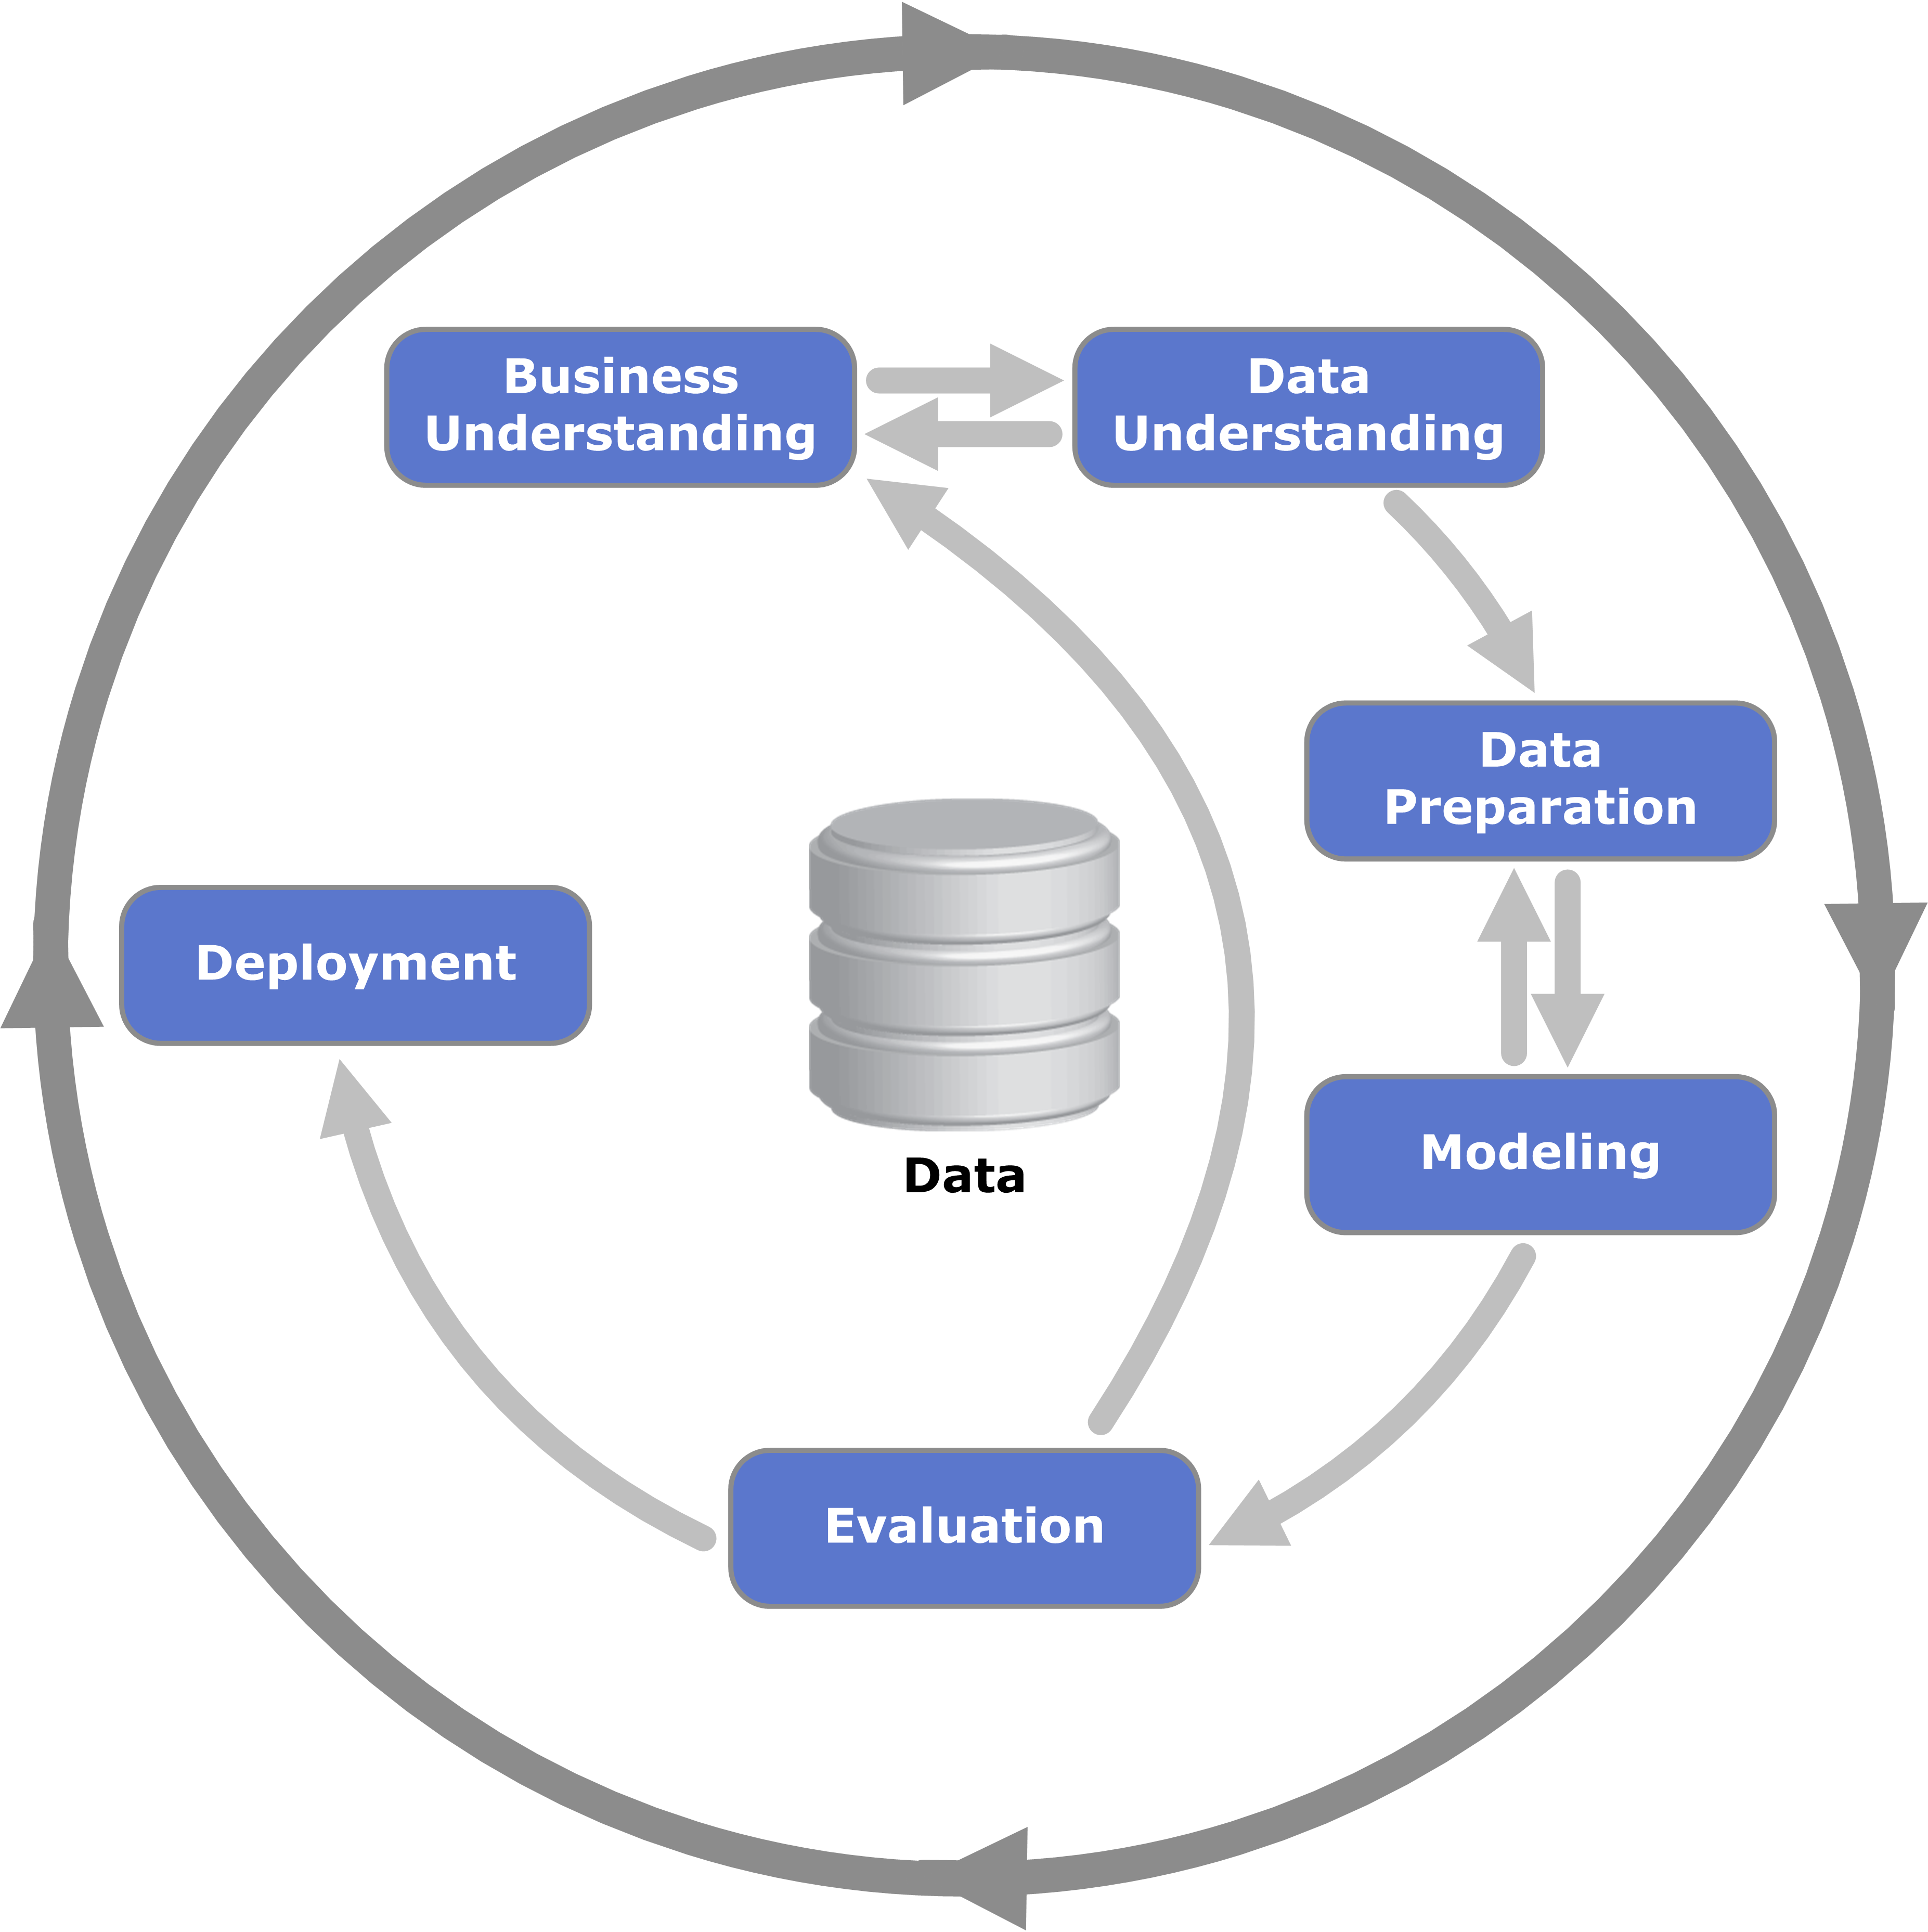
\includegraphics[width=0.5\linewidth]{./images/CRISP-DM.png}
	\caption{CRISP-DM}
	\label{fig:crispdm}
\end{figure}

\subsubsection{Business Understanding}
Utilizing obstacle detection with computer vision can play a crucial role in helping various enterprises address concerns with regards to safety. Our goal is to create a lightweight model that can be embedded on vehicles such as drones. Companies that focus in industries that require lightweight models that can predict in real time, such as autonomous vehicles, railroads, and robotics can use this idea to detect any obstacles in real time. This helps prevent severe accidents from occurring. It also allows drivers to focus on the road without having to also detect whether anything comes in the way. Having this extra safety mechanism can help to increase a human's trust and reliability on the product if using something like autonomous vehicles since it ensures the customer that extra safety precautions are being taken. If accidents occur, time and money must be spent for repairs, while at the same time inconveniencing unrelated parties. Having a quick and accurate obstacle detection mechanism in place can identify potential obstacles and help prevent accidents from occurring.


\subsubsection{Data Understanding}
For the data collection phase, the primary datasets will be sourced from public repositories such as the COCO dataset, RoboFlow, and other APIs that are focused on obstacle detection across various domains (Mainly on Autonomous drones). The custom datasets will also be created and used by capturing images and videos in various environments.

For the data exploration phase, we are going to conduct an initial EDA process to assess the distribution of the class, such as car, pedestrian, and more. Another important aspect of our data that we need to understand is its format. For example, YOLOv11 and RT-DETR can use JPEG and PNG images with JSON annotations, while Detectron2 supports JPEG, PNG, and TIFF image formats, also using JSON annotations. It is essential that the data format is known, because the data will be combined into one master dataset. One issue that arises when doing so is differing formats among the data. As stated before, certain architectures are able to handle certain image types, label formats, etc. Additionally, data often come in different formats, such as image size, colorspace, image type, and annotation format. Due to this, we must understand the data formats first to ensure consistency when we combine our data together.


\subsubsection{Data Preparation}
The dataset can consist of a set of images or videos. Since our datasets will be combined into one master dataset, the data must be consistent across all datasets. For any videos in the dataset, we can convert them into images by splitting it into frames. Then, we will resize the images to be the same size, as differing sizes will cause issues with modeling. Next, we will ensure each image is in the same colorspace by changing the color representation so that each pixel is either in a black and white format or in an RGB (Red, Green, Blue) scale representation. Additionally, we will convert all of the images to the majority image type.

Once this is done, the data can be preprocessed to increase robustness, as well as to increase the model's performance.
Images within the dataset can be cropped to eliminate parts that are irrelevant to the detection process. Rotation and flipping will be applied to obtain additional training data in different orientations. We will try normalizing certain pixel values which can help keep the components of the image on one scale and help the model reach the optimal solution faster. In case any unnecessary components are discovered, we can apply masking so the model only focuses on the relevant parts. In a similar project using YOLOv8 to detect moving objects conducted by \textcite{safaldin_improved_2024}, preprocesses a video, by decoding it which required them to ``isolate each frame from the video'', making adjustments to the size of each frame since ``YOLO architectures require certain input sizes'', and adjusting the color by transforming ``pixel values to a range between to [0, 1] or [-1, 1]'' depending on the model used.

% *** https://docs.opencv.org/4.x/d2/d96/tutorial_py_table_of_contents_imgproc.html *** this just has some stuff that opencv can do in terms of image preprocessing

\subsubsection{Modeling}

In the model selection phase, the project is primarily implemented by three different well-known object detection model architectures, which are YOLOv11, Detectron2, and RT-DETR. The YOLO architecture is a popular real-time object detection model with high speed and accuracy, which makes it suitable for a real-time detection application. Detectron2 is developed by Facebook AI Research, and the main advantage is the flexibility of selecting various backbone networks and the robustness of the model performance. Finally, RT-DETR is a transformer based model, designed for real time prediction. The advantage of a transformer based model is that it is able to better detect small or occluded obstacles.

During the model training phase, these selected architectures will be trained and optimized for the obstacle detection tasks outlined in the project. Initially, transfer learning will be utilized by leveraging weights from a pre-trained model that have been trained on larger datasets such as COCO. This will allow models to preserve some important features while reducing the time and data required for training. Additionally, fine tuning these models may be required depending on the performance.



\subsubsection{Evaluation}
To evaluate the performance of each model, there are different techniques available to use. To compare the effectiveness of each YOLO model, \textcite{quach_evaluating_2023} utilize measurement scales such as Average Precision (AP) to help identify how well the model detects various objects. They also other standard evaluation metrics such as precision, recall, and F1-score to determine the model's performance in order to identify with how much certainty it can classify a certain image. Their evaluations are based on an ``Intersection of Union threshhold (IoU) or ground truth ratio to confirm whether the recognized object is true or false'' \parencite{quach_evaluating_2023}. We will obtain the precision, recall, and f1-scores to evaluate the model performance. Using the precision values, we will also calculate the mean average precision. This metric is considered as the ``consolidated metric for assessing model accuracy across varying categories and confidence levels'' \parencite{safaldin_improved_2024}. Alongside that, we will determine the Intersection of Union to determine how much similarity there is between the actual label and the predicted label. Lastly, the inference time is a key evaluation metric. Since our end goal is an embedded model, real time predictions are required. The inference time will be measured in Frames Per Second (FPS), which represents the number of image frames the model can process in a second.

\subsubsection{Deployment}
The product deployment will consist of the model that detects obstacles and objects the most accurately while taking into account the inference time. The model will be trained on a dataset related to typical obstacles and viewpoints from a drone's perspective. For now, the VisDrone dataset is used.


\subsection{Data Pipeline Architecture}
% data sources, data warehouse, ETL, ELT, data transfers with pipeline, and deliverables

% data source aside, do we even have a start for the other steps
For this project, the image data and labels will be sourced from previously established datasets with research, such as the COCO dataset, as well as more targeted data from online aggregates like Roboflow. This data will then be stored in an AWS S3 bucket. For ETL and pipelining, we will focus on extracting the data from the bucket, transforming them to a single format (image type, image size, colorspace, etc.), then loading it into the data warehouse.

\subsection{Project Organization Plan}
To organize the project, a work breakdown structure was creating by decomposing the project hierarchically and incrementally into phases, deliverables, and work packages. The phases, deliverables, and work packages are as follows:

\begin{enumerate}
	\item Business Understanding: This phase is split into four main work packages: Defining the problem, performing literature and technology surveys on the topic, determining the data source, and creating the project plan framework.

	\item Data Understanding: This phase it split into two packages: Understanding the image data and initial exploratory data analysis. Understanding the image data is a hierarchical system, where the sub packages involves understanding the format of the data, as well as understanding the images themselves in terms of factors such as image size, colorspace, and image type.

	\item Data Preparation: This phase involves two packages: Preparing the data and Splitting the data. Preparing the data is split up into various, incremental tasks: Collecting the data, reformatting the data to be consistent with each other, cleaning the data, transforming and augmenting the data, and labeling the data if needed. Once this is done, we can split the data into train, validation, and testing sets.

	\item Modeling: The modeling phase has 3 main packages: Model Research, Modeling and Validation, and Evaluation. Model Research is split into 3 sub tasks: researching YOLOv8, Detectron2, and RT-DETR. Once this is completed we can move on to the modeling and validation step, where these architectures will go through transfer learning and fine tuning. Finally, we can evaluate the models by comparing their performances, and select the best performing one.

	\item Deployment: The deployment phase has two deliverables: Deploying the project and data onto AWS as a backend prototype, and the final report submission.
\end{enumerate}

The rough work breakdown structure can be seen in Figure \ref{fig:wbs}.
\begin{figure}[!htb]
	\centering
	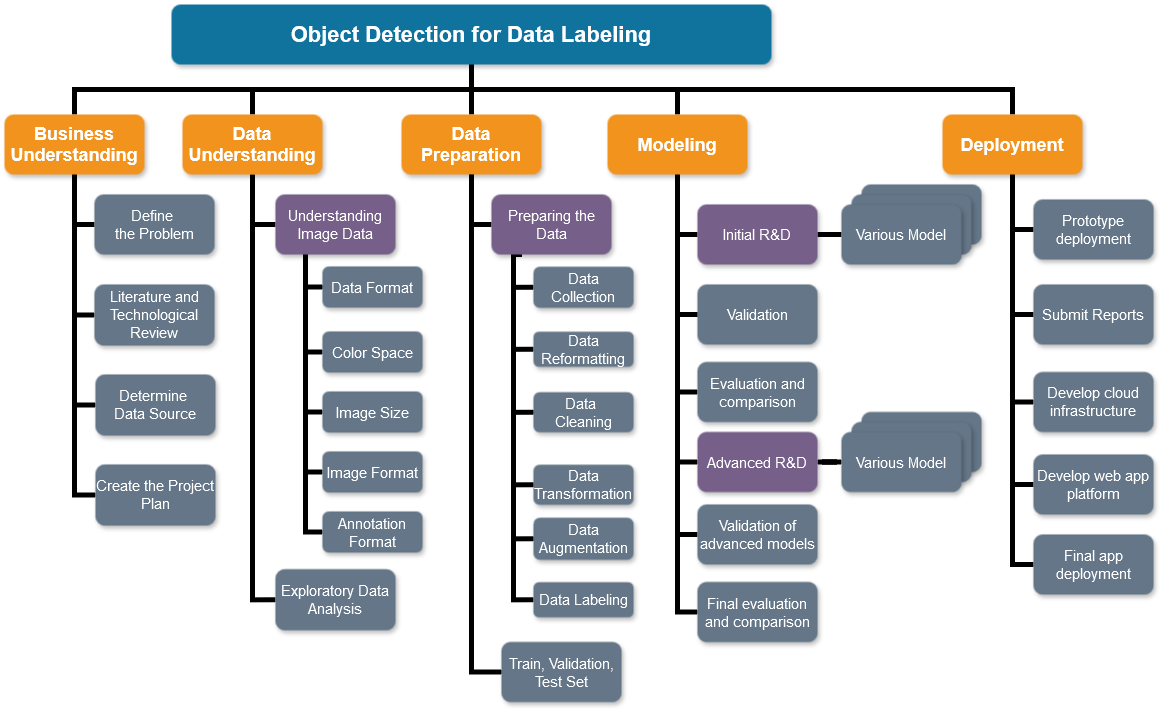
\includegraphics[width=1\linewidth]{./images/WBS.png}
	\caption{Work Breakdown Structure}
	\label{fig:wbs}
\end{figure}


\subsection{Project Resource Requirements and Plan}
\subsubsection{Hardware}
Deep learning is generally computationally intensive, especially when performing it on images. As a result, we require more powerful hardware. The main pieces of hardware we plan to utilize are our own local machines and Google Colab. A summary of our hardware requirements can be seen in Table \ref{tab:hardware}.

We plan on utilizing Google Colab for initial testing. Google Colab is a free-to-use, cloud-based Jupyter Notebook with access to GPU and TPU resources. The free-to-use version has limited resources, so depending on the process, a paid plan may be required. Additionally, Google Colab is integrated with Google Drive, allowing data storage and collaboration through the use of shared drives.

\begin{table}[!htb]
	\centering
	\caption{Hardware Requirements}
	\begin{tabular}{cccc}
		\hline
		Service        & Configuration     & Purpose          & Cost         \\
		\hline
		Local Machines & various           & Coding platform  & Owned (free) \\
		Google Colab   & T4 GPU (16GB RAM) & Compute platform & Free         \\
		\hline
	\end{tabular}
	% \tablenote{*Paid version available, A100 GPU utilizes approximately 11 compute units/hour}
	\label{tab:hardware}
\end{table}

\subsubsection{Software}
To preprocess the data and create the models, various software tools must be utilized. The primary coding language will be Python. In addition to Python, various libraries and modules related to modeling and data preprocessing will be used. We also use GitHub and Google Colab for collaborative coding, and Google Docs and Overleaf for report writing A comprehensive list of the software used can be seen in Table \ref{tab:software}.

There are no specific licenses require for the aforementioned tools and platforms. The majority of these tools are open-source, or have free versions for both personal and academic use. Businesses and organizations may have different requirements such as having to purchase licenses, but this does not apply for our use case.

\begin{table}[!htb]
	\centering
	\caption{Software Requirements}
	\begin{tabular}{cccc}
		\hline
		Service          & Configuration  & Purpose                      & Cost      \\
		\hline
		Python           & Version 3.11   & Coding platform              & Free      \\
		Pandas           & Version 2.1.1  & Working with datasets        & Free      \\
		NumPy            & Version 1.26.1 & Advanced mathematics         & Free      \\
		PyTorch          & Version 2.4    & Modeling, Data Preprocessing & Free      \\
		OpenCV           & Version 4.10   & Image Processing             & Free      \\
		Ultralytics      & Version 8.3.2  & Modeling (with YOLOv11)       & Free      \\
		Detectron2       & Version 0.6    & Modeling (with Detectron2)   & Free      \\
		Jupyter Notebook & Version 6.5.4  & Code REPL platform           & Free      \\
		Google Colab     & N/A            & Code REPL platform           & Free      \\
		Kaggle Notebook  & N/A            & Code REPL platform           & Free      \\
		GitHub           & N/A            & Code collaboration           & Free      \\
		Overleaf         & N/A            & Report writing collaboration & \$9/month \\
		TeamGantt        & N/A            & Gantt charts                 & Free      \\
		\hline
	\end{tabular}
	% \tablenote{*Paid version available}
	\label{tab:software}
\end{table}

\subsection{Project Schedule}

Project management is required to make sure projects are completed on time. To do so we use the waterfall technique to task management and to keep up with it we are following a schedule. This schedule can be visualized as a Gantt chart or PERT chart. A Gantt chart shows the tasks on a timeline with dependencies, resources, and durations clearly visible. It allows for quick references to make sure we are on track. A PERT chart allows us to find the critical path in a projects completion. If there is a delay in any of the tasks in the critical path, that means there will be a delay on the entire project.

Based on our project organization plan, the project schedule can be broken down into the same phases, namely; business understanding, data understanding, data preparation, modeling, and deployment. We created a Gantt chart to visualize this schedule and help use stay on track. Figure \ref{fig:gantt_1} shows our schedule for our research phase, which involves reading papers, doing comparative analysis, and selecting the appropriate approaches.

\begin{figure}[!htb]
    \centering
    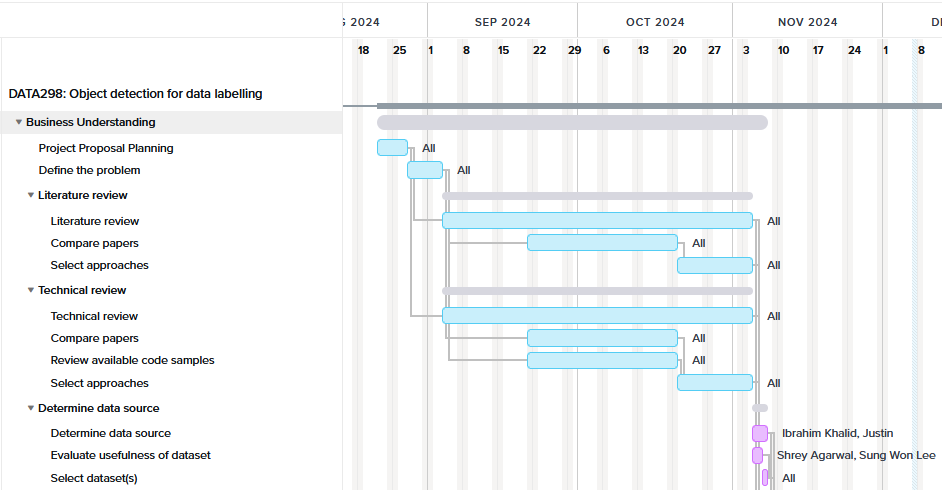
\includegraphics[width=\linewidth]{images/gantt/gantt_1.png}
    \caption{Project schedule, Business understanding}
    \label{fig:gantt_1}
\end{figure}

Figure \ref{fig:gantt_2} shows the data phase of our project where we mainly focus on finding out the properties of the images in our dataset and the special considerations we need to make in our model regarding them. Since we have multiple models, we also spend time making sure that the same dataset is compatible with all models. If they are not compatible, then we must create a function to do those conversions for us. The rest of the time in this phase focuses mostly on data cleaning, images transformations, augmentations, and labeling. 

\begin{figure}[!htb]
    \centering
    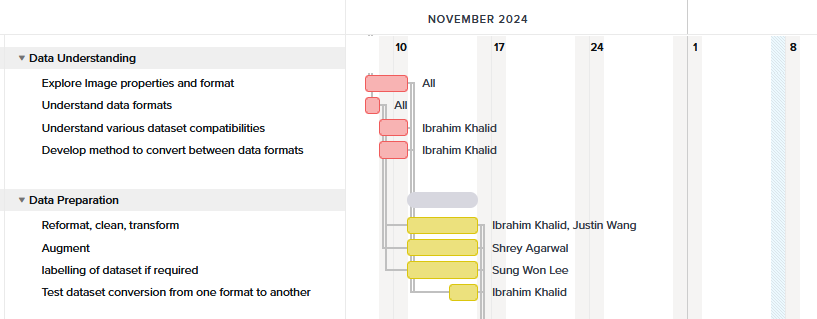
\includegraphics[width=\linewidth]{images/gantt/gantt_2.png}
    \caption{Project schedule, Data understanding and preparation}
    \label{fig:gantt_2}
\end{figure}

The most important phase of the project is during the modeling phase where we will take our selected models and train them on our selected datasets, configuring them to make sure they work as intended and produce good results. Simultaneously, we develop a pipeline version of atleast one model to run entirely on the cloud.

\begin{figure}[!htb]
    \centering
    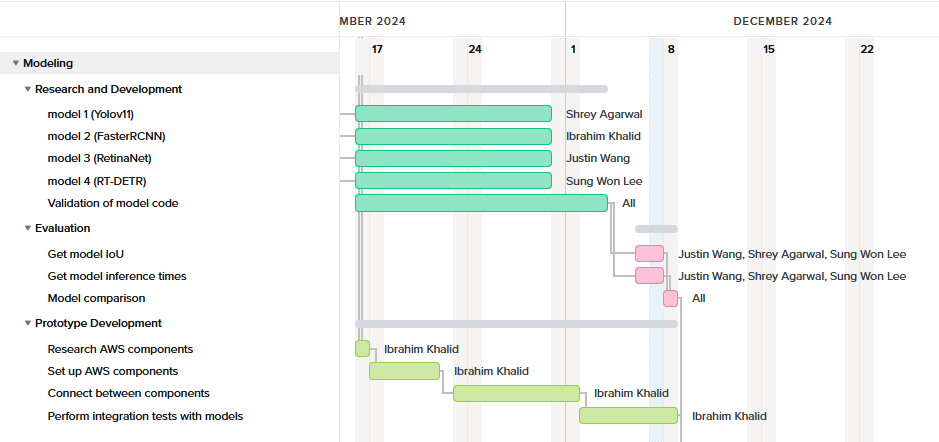
\includegraphics[width=\linewidth]{images/gantt/gantt_3.png}
    \caption{Project schedule, Modeling and prototype deployment}
    \label{fig:gantt_3}
\end{figure}


\begin{figure}[!htb]
    \centering
    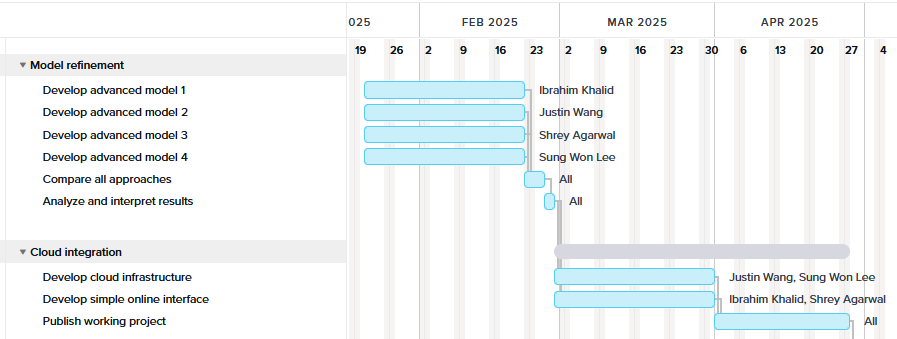
\includegraphics[width=\linewidth]{images/gantt/gantt_4.png}
    \caption{Project schedule, tentative semester 2 schedule}
    \label{fig:gantt_4}
\end{figure}


\section{Data Engineering}
\subsection{Data Process}
The dataset used will be the VisDrone dataset. Due to the way the data pipeline is structured, this dataset is obtained from the Ultralytics GitHub. The data is passed through the pipeline to format it into YOLO format and COCO JSON format. Once this reformatting is completed, we download the data as a zip file. For more information, see the Data Pipeline section later in this report.

After obtaining the data, we will perform image augmentations such as flipping, rotation, and color jittering to change the hue, saturation, and brightness of the images to emulate various environmental conditions. Once this is done, we will split the data into training, validation, and testing sets with a split of 80-10-10. Finally, we look at some statistics of the dataset.

\subsection{Data Collection}
The data is the VisDrone dataset. It consists of 288 video clips with 261,908 frames and 10,209 static images from various drone-mounted cameras. The dataset showcases varying cities in China, urban and rural communities, various objects, and different level of crowd density. Due to the current limitations of the data pipeline, we are working with only the training dataset of the VisDrone data, and are splitting that into train, validation, and test. For more details, see the Data Pipeline section.
The data taken contains 6471 images and their associated labels, with the following 10 classes:
\begin{itemize}
	\item Awning-Tricycle
	\item Bicycle
	\item Bus
	\item Car
	\item Motor
	\item Pedestrian
	\item People
	\item Tricycle
	\item Truck
	\item Van
\end{itemize}

% Present samples from raw dataset (before preprocessing)
%%% images

The images found in Figure \ref{fig:sample_images} show examples from our raw dataset.
\begin{figure}
	\centering
	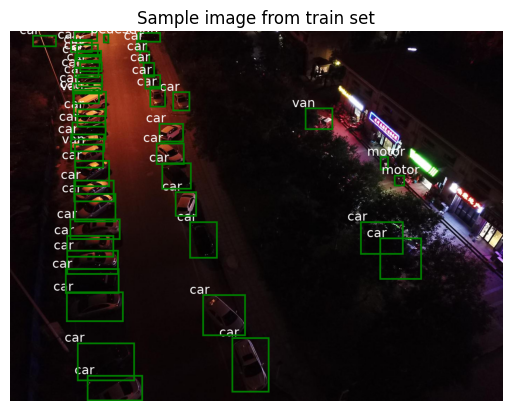
\includegraphics[width=0.33\linewidth]{images/sample_train.png}
	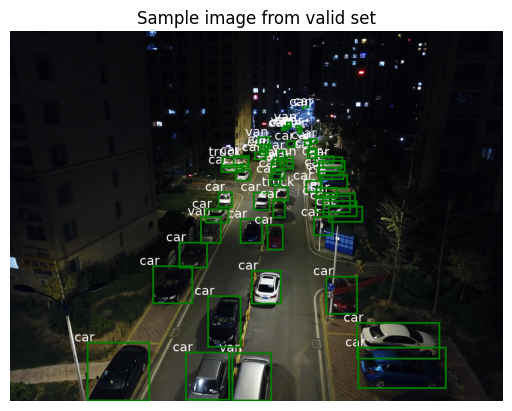
\includegraphics[width=0.33\linewidth]{images/sample_valid.png}
	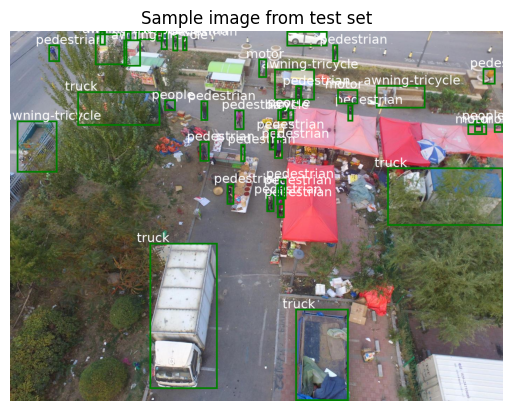
\includegraphics[width=0.32\linewidth]{images/sample_test.png}
	\caption{Sample images from each split}
	\label{fig:sample_images}
\end{figure}


\subsection{Data Pre-processing}
For image data, preprocessing and transformations go hand in hand. We define image preprocessing as changing the qualities of the image without changing its orientation. As an example of a transformation, flipping the image is used to increase the robustness of the data through changing its orientation.

As such, our preprocessing steps include resizing the image, normalizing the image, and using color jittering. Resizing an image is helpful for a multitude of reasons. Depending on the size of the image, it can increase or decrease the efficiency of the model. We downsize the images to improve the efficiency of the model while still maintaining its important features. In the case for YOLO, we resized the images to 640x640 as this is one of the common values used.

Normalization is used for many reasons. The first reason is to scale each pixel value of our image down, allowing for models to learn quicker and keeping weight updates smaller which helps with gradient descent. We used a mean and standard deviation of 0.5 to normalize our pixel values to a value between -1 and 1.

Color jittering is used to change the hue, saturation, and brightness of an image. In our case, color jittering is used to try to emulate environmental conditions, such as day and night, snow, rain, and so on. We adjust the hue, saturation, and brightness of our images by 0.015, 0.7, and 0.4 respectively.



\subsection{Data Transformation}
After the dataset has been pre-processed, we proceeded with the data transformation process. we have applied several transformation techniques to increase the robustness and the diversity of the training images. The major transformation tasks include translation, rescaling, and mirroring.

For the translation, it shifts the image horizontally and vertically by a fraction of the image size which allows the model to detect objects positioned in various parts of the frame or even partially visible. Here, we set the variable to be 0.1 which means that the training image will be shifted by 10\% of its image size.

In the case of rescaling, it augments the image by simulating objects at different distances from the camera. Thus, it helps to standardize the size of the object in the image, which make the model to detect the object regardless of the object size. In our model, we set the parameter to be 0.5, which means it gives 50\% variation on scaling to zoom in or out on the object.

Mirroring, or flipping left and right, is used to flip the image. This is done to give more representations for the same data, increasing the dataset's diversity. For our use case, we set the parameter to be 0.5, meaning that this augmentation is applied 50\% of the time.

Figure \ref{fig:sample_images_transformed} shows examples of our images after the above transformations are applied.
\begin{figure}
	\centering
	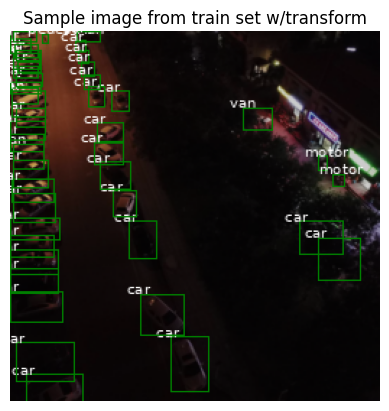
\includegraphics[width=0.33\linewidth]{images/sample_train_t.png}
	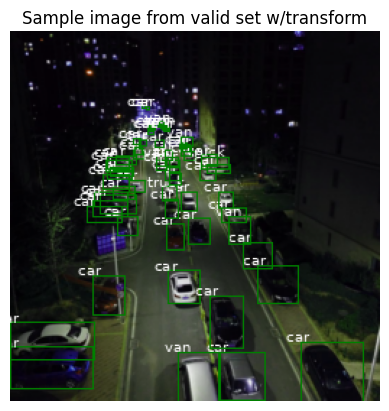
\includegraphics[width=0.33\linewidth]{images/sample_valid_t.png}
	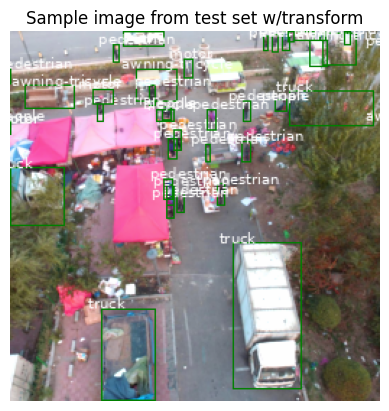
\includegraphics[width=0.32\linewidth]{images/sample_test_t.png}
	\caption{Sample images from each split with transformations applied}
	\label{fig:sample_images_transformed}
\end{figure}


\subsection{Data Preparation}
Once the data has been pre-processed and transformed, we will split it into a train, validation, and test set. The validation set will be used to help better tune the model for training. We will be splitting the data into 80 percent training, 10 percent validation, and 10 percent testing. In this case, our dataset of size 6471 is split into a training set of size 5176, a validation set of size 647, and a testing set of size 648. Samples of the data can be seen in Figure \ref{fig:sample_images_transformed}.

\subsection{Data Statistics}
For image data, there is not much in the way of statistics. However, we did find some facts about the dataset just to get a feel for it. These facts can be seen in Table \ref{tab:facts}. These facts show that the typical size of a bounding box is very small and there are many of them per image. This may pose a challenge for us in training. In Figure \ref{fig:cls_distrib}, we show the distribution for each class by train, validation, and test split. We note that it seems like "car" is the most common label, while awning tricycles are the least common. For validation and test, the distributions seem to be even.

\begin{table}[!htb]
	\centering
	\begin{tabular}{lr}
		\hline
		\textbf{Metric}                             & \textbf{Value}                         \\
		\hline
		Average image area                          & 1,573,546.484006 px\textsuperscript{2} \\
		Average bounding box area                   & 2,493.606550 px\textsuperscript{2}     \\
		Ratio of bounding box area to image area    & 0.158470\%                             \\
		Average number of classifications per image & 53                                     \\
		\hline
		\textbf{Image sizes}                        &                                        \\
		\hline
		Maximum image size                          & 3,000,000 px\textsuperscript{2}        \\
		Minimum image size                          & 172,800 px\textsuperscript{2}          \\
		Most common image size                      & 1400 x 1050 px\textsuperscript{2}      \\
		\hline
		\textbf{Bounding box sizes}                 &                                        \\
		\hline
		Maximum bounding box size                   & 329,847 px\textsuperscript{2}          \\
		Minimum bounding box size                   & 4 px\textsuperscript{2}                \\
		Most common bounding box size               & 11 x 11 px\textsuperscript{2}          \\
		\hline
	\end{tabular}
	\caption{Dataset facts}
	\label{tab:facts}
\end{table}



\begin{figure}[!htb]
	\centering
	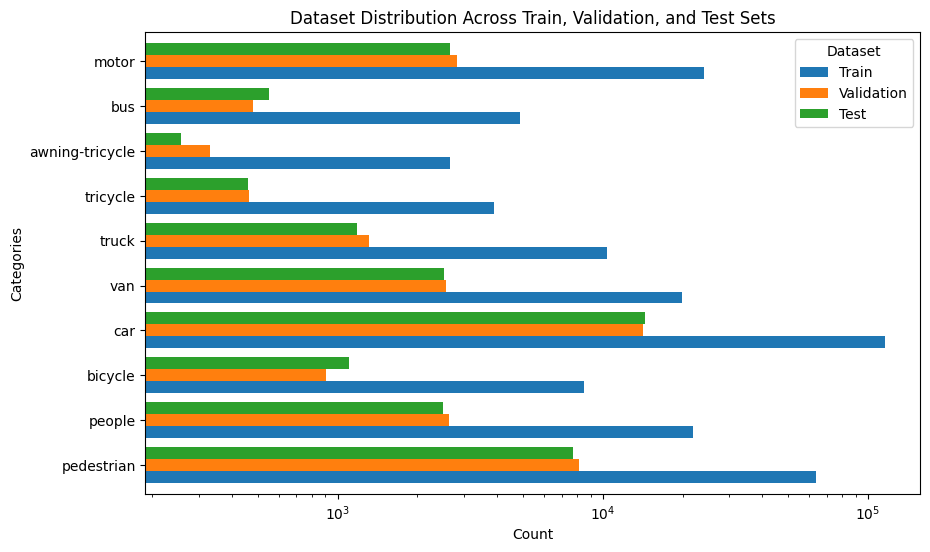
\includegraphics[width=0.75\linewidth]{class_distribution.png}
	\caption{Class Distribution by Split}
	\label{fig:cls_distrib}
\end{figure}

\section{Model Development}
\subsection{Model Proposals}
For modeling, we will be using transfer learning on state of the art object detection systems. The first of which is YOLO, which is based on single shot detection. It uses a single pass of the input image to perform classification and localization. For YOLO, it divides the image into a grid and predicts bounding boxes and class labels for each grid, then filters them out based on factors such as confidence and Intersection over Union. YOLO has different versions, each with slightly different architectures to improve speed and performance.

Detectron2 on the other hand, is based on two shot detection algorithms such as Faster RCNN and Mask RCNN. It utilizes a CNN backbone with a feature pyramid network, creates regions of interest using a region proposal network, then passes these in to region of interest heads to make predictions.

According to \textcite{yaseen_what_2024},  YOLOv8 is a single-shot detector that processes the entire image in one pass, which make YOLOv8 possible to handle both classification and localization within each grid cell. The backbone of YOLOv8 is a advanced convolutional Neural Network and the neck of YOLOv8 architecture uses Feature Pyramid Networks (FPN) integrating with Path Aggregation Network (PAN) structure, which allows the model to handle multi-scale feature extraction from the input image. This architecture aggregates the features from multiple layers, ensuring that both high and low level features also be used in the final prediction. Finally in the head part of the architecture, it generates final prediction including bounding box coordinates, confidence scores, and class labels. The key features of YOLOv8 is that unlike typical object detection models, YOLOv8 adopts an anchor free approach. Instead of predefining anchor boxes, it directly predicts bounding boxes, which simplifies the complexity and improves detection accuracy for irregularly shaped objects. Pictured in Figure \ref{fig:YOLOv8-architecture} is the architecture for YOLOv8.

YOLOv11 is similar in concept for YOLOv8. According to the Ultralytics documentation \parencite{yolo11_ultralytics}, YOLOv11 has enhanced feature extraction due to its improved backbone and neck, better speed and efficiency due to its new architectures and pipelines, and fewer parameters than its previous versions while having better accuracy. Rather than the C2F blocks that YOLOv8 uses, YOLOv11 replaces them with C3k2 blocks, which are an improved version of the C2F block in terms of feature representation and efficiency due to its usage of split feature maps and smaller kernel sizes. Additionally, YOLOv11 adds an attention mechanism, known as the C2PSA block, to the end of its backbone; something that was non existent in previous versions. Due to the improved performance of YOLOv11, we chose to use it over previous YOLO models.

Unlike YOLO, Detectron2 is uses two shot detection, meaning that its first pass generates regions of interest, and the second pass refines the proposals, extracts features, classifies, and creates bounding boxes for those regions. Detectron2 is primarily based on Mask RCNN, which is an extension of Faster RCNN. In this implementation, an input image is passed through a CNN backbone to extract its features. Then, this feature map is first passed into the region proposal network to obtain regions of interest, and both the feature map and regions of interests are passed into an RoI pooling layer to extract features from the regions of interest. For the typical Faster RCNN, the output from the RoI pooling layer is passed in to fully connected layers, outputting bounding box coordinates and their associated labels. For Mask RCNN, the feature map is also passed into another CNN to generate segmentation masks. Figure \ref{fig:Detectron2-architecture} features the basic architecture for Detectron2.

%
Real Time Detection Transformer, better known as RT-DETR, is a transformer based object detector that provides real time performance with relatively high accuracy. As the name suggests, it is based on the DETR framework, which is non-maximum suppression free. The paper notes that the speed and accuracy of typical YOLO models are negatively affected by NMS. To improve its processing speed, RT-DETR utilizes a convolution based backbone and a hybrid encoder. By leveraging these attributes, RT-DETR is able to efficientl process multiscale features by decoupling intrascale interaction and cross scale fusion to improve speed. Additionally, the model supports flexible speed tuning by allowing for the adjustment of the number of decoder layers to adapt to situations. The basic architecture for this model can be seen in Figure \ref{fig:rt-detr}.


The models we will be using are as follows: YOLOv11, Detectron2 using Faster RCNN and RetinaNet, and RT-DETR. For future tests, we will test with different architecture sizes for YOLO and different models for Detectron2 from the model zoo featured on their GitHub page, since each architecture has its own advantages and disadvantages.

\begin{figure}[!htb]
	\centering
	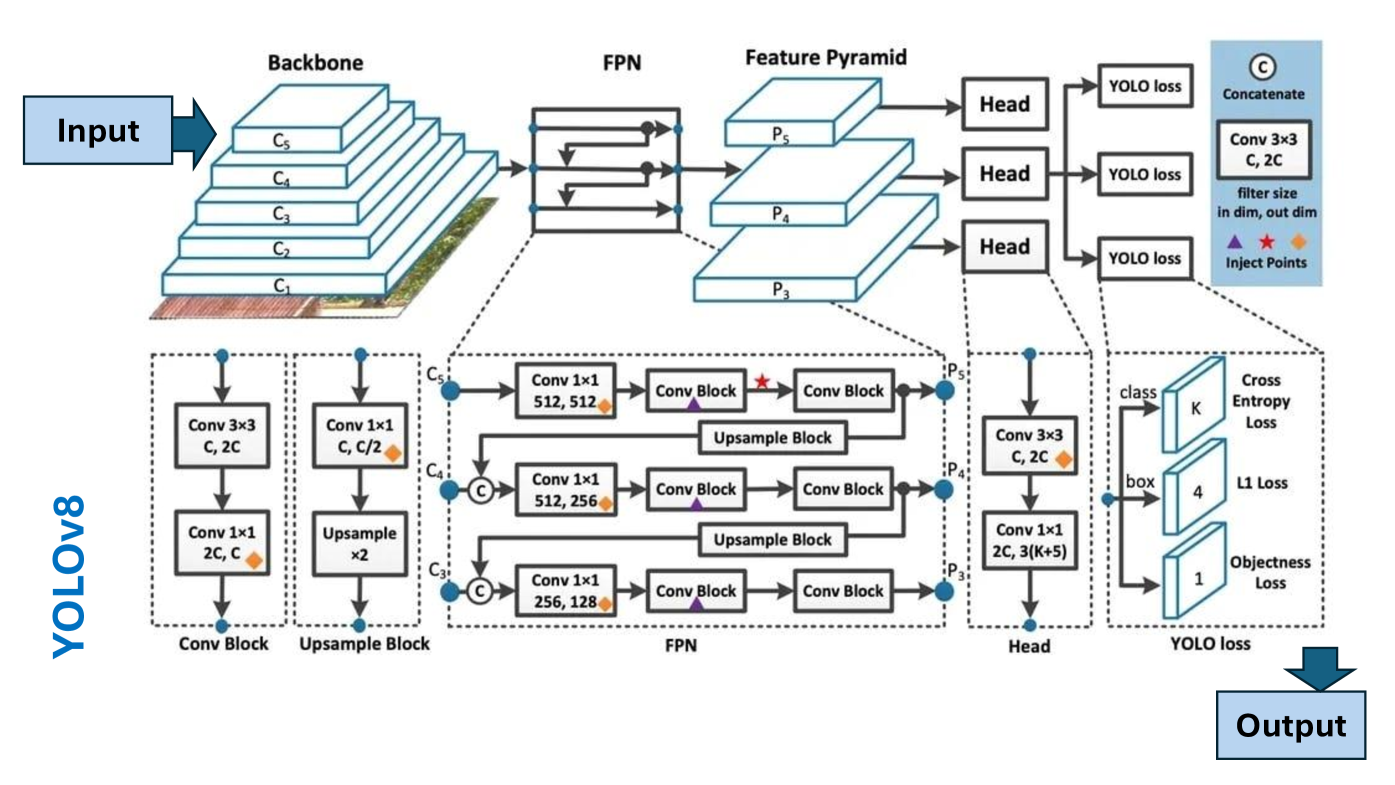
\includegraphics[width=0.75\linewidth]{images/YOLOv8_architecture.png}
	\caption{Basic architecture of YOLOv8.
		\textit{Note}. The figure is taken from \textcite{sapkota_comparing_2024}}
	\label{fig:YOLOv8-architecture}
\end{figure}

\begin{figure}[!htb]
	\centering
	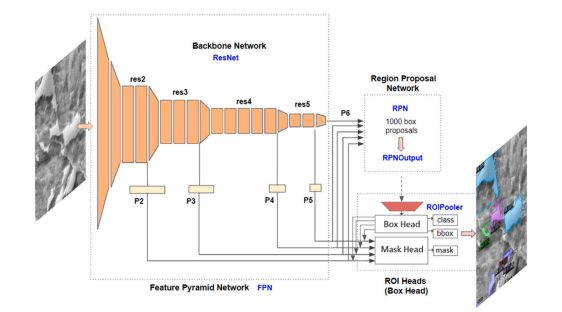
\includegraphics[width=0.75\linewidth]{images/Detectron2_architecture.png}
	\caption{Basic architecture of Detectron2. \textit{Note}. The figure is taken from \textcite{ackermann_automated_2022}}
	\label{fig:Detectron2-architecture}
\end{figure}

\begin{figure}
    \centering
    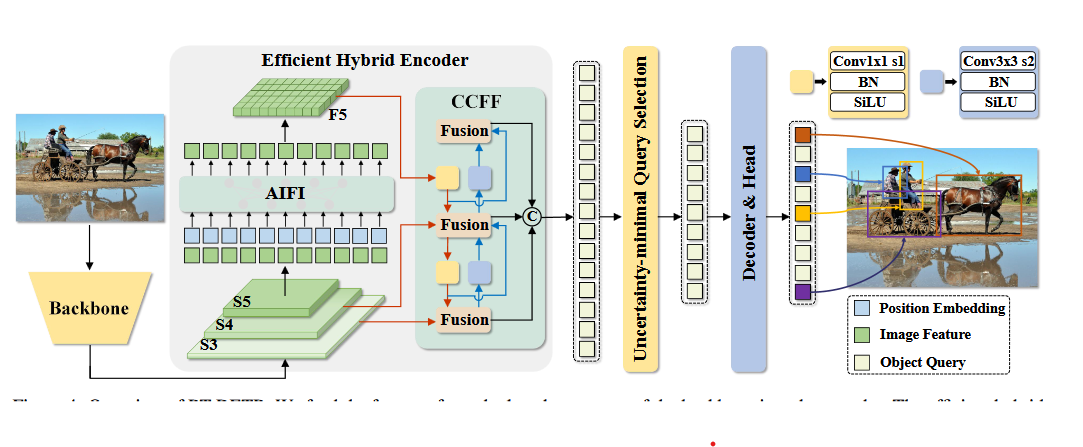
\includegraphics[width=0.75\linewidth]{rt-detr_architecture.png}
    \caption{Basic architecture of RT-DETR}
    \label{fig:rt-detr}
\end{figure}


\subsection{Model Supports}
Given the high computational demands of deep learning tasks with image data, especially complex models such as YOLO, RT-DETR, and Detectron2, where it mandatorily requires GPU computational power, access to environments with robust GPU resources is important for efficient model training and evaluation. For this project, we will primarily be using Google Colab and Kaggle Notebooks due to their free GPU access, which accelerates the training and testing of our models.


\subsubsection{Hardware environment}
For the hardware environment, Google Colab provides access to NVIDIA T4 GPU, which enable us to have strong performance for deep learning tasks, especially for large image datasets. Also, Kaggle notebook offers NVIDIA P100 GPU, which allow us to handle complex and computationally heavy models such as YOLO and Detectron2. Kaggle notebook has 30 hours of free GPU usage that refreshes every week. This makes it a useful tool when taking into consideration the computational cost of the models.

\subsubsection{Frameworks}
For frameworks we are using, both Google Colab and Kaggle Notebooks support PyTorch and TensorFlow. Thus, for this project, we will primarily use PyTorch due to its flexibility and compatibility with the obstacle detection task. We will also use the Ultralytics YOLO library, which integrates smoothly with PyTorch, so that it makes training and deploying the YOLO and RT-DETR models simpler.


The figure \ref{fig:mlFlowchart} represents general platform architecture view from VisDrone dataset to model evaluation. The pipeline begins with the VisDrone Dataset and go through the data pipeline and stored in an AWS S3 bucket. Then four models are trained on the processed data. The training process is proceeding in Google Colab and Kaggle Notebook. Finally, models will be optimized and we can evaluate the model from the results we get.

\begin{figure}[!htb]
	\centering
	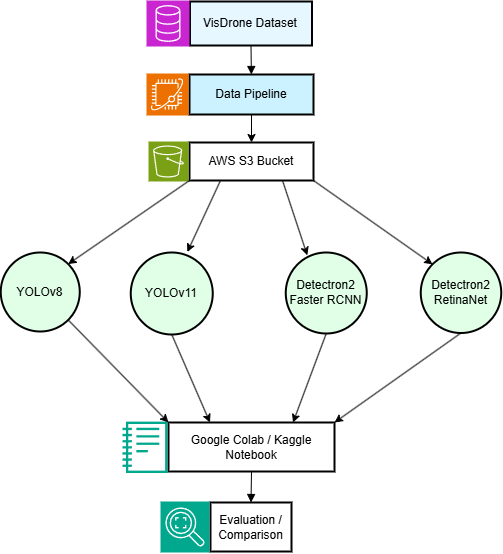
\includegraphics[width=0.6\linewidth]{images/modelsupportDiagram.png}
	\caption{Platform architecture and model flowchart}
	\label{fig:mlFlowchart}
\end{figure}


\subsection{Model Comparison and Justification}

The primary targeted problem is to detect obstacle efficiently and accurately in various challenging environments especially in drone path domain. The models considered include YOLOv11, Detectron2, and RT-DETR.

As mentioned in the model proposal section, YOLOv8 is a single shot detector built upon Convolutional Neural Network and Feature Pyramid Network combined with Path Aggregation Network for the purpose of multi-scale feature extraction. YOLOv11 has similar architecture to YOLOv8, but it replaces C2F block in YOLOv8 with more efficient C3k2 blocks so that it can reduces parameter count while boosting a speed. On the other hand, Detectron2 uses a two-shot detector built upon Mask RCNN. It uses Convolutional Neural Network, Region Proposal Network as backbones and uses RoI pooling to identify object locations.


\subsubsection{Strengths and Limitations}
Based on the findings of multiple studies, each model shows different strengths and limitations. YOLOv8 generally shows high speed and efficiency due to its single-shot detectors, makes tasks that requires rapid object detection such as real-time video or image analysis easier. However, while YOLOv8 has strong strength on its speed, the accuracy may be lower than the complex models such as Detectron2. This may result in limiting the applications where precise object detection is required.

Due to its more lightweight nature, YOLO models tend to be much faster than the likes of Detectron2. However, this speed sacrifices some of its peformance. Both YOLOv8 and YOLOv11 share these strengths and limitations, but YOLOv11, due to its improved architecture, boasts greater speed and performance.

On the other hand, due to its two-shots detectors which include RPN, this aspects make Detectron2 as well known for its high accuracy, especially in tasks that need to segment or detect detailed objects where the objects are densely packed. However, this strength of precision and accuracy comes at the cost of slower inference times compared to YOLO models because of its complex architecture.

\textcite{wadhwa_comparison_2023} compares the performance of YOLOv8 and Detectron2 on crowd counting techniques. They found that while Detectron2 had better accuracy, YOLOv8 was able to detect more objects. Furthermore, YOLOv8 was faster in terms of computation time. This means that there is a trade off between performance and speed.

This concept can be extended to YOLOv11, which is a newer version than YOLOv8. In other words, YOLOv11 should also have the performance vs speed trade off when compared to Detectron2. While it may seem like YOLOv11 is better than YOLOv8 in every way given that it is the newer version, this is actually not the case.

According to the research of \textcite{sapkota_comparing_2024}, the author compares YOLOv11 and YOLOv8 on the segmentation task, the result shows that YOLOv11 illustrates better performance overall, but YOLOv8 has a slightly faster inference time.

On the other hand, in the research, \textcite{alif_yolov11_2024}, it also compares YOLOv11 with YOLOv8 and the result showed that YOLOv11 outperformed YOLOv8 across every metrics.

\subsubsection{Justifications for Model Selection}

According to the existing research elaborated on the previous section, YOLO models show relatively better performance on detecting high number of objects efficiently, while Detectron2 demonstrates relatively better accuracy, particularly in more complex environments. However, there are some contradictory results between the performance of YOLOv8 and YOLOv11 that we wanted to confirm. Thus, by experimenting with YOLOv8, YOLOv11, and Detectron2, we aim to check whether these results on the research hold true in our specific application domain so that we can select the model for our final deployment that best aligns with the real-time processing needs and accuracy.

Detectron2 has different backbone architectures available in their model zoo. We chose to use RetinaNet as one backbone due to its speed and accuracy. RetinaNet, however, is also a one shot detector, just like YOLO. Due to this, we also chose to use Faster RCNN as the backbone because of its nature as a two shot detector.

\subsection{Model Evaluation Metrics}
For this research, we will be using basic evaluation metrics commonly used for object detection tasks. These are mean average precision (mAP) and intersection over union (IoU).

Mean Average Precision: To understand mAP, we need to first understand what average precision is. Average precision is calculated as the weighted mean of precisions for each given threshold; in other words, it computes the area under the precision-recall curve. This combines the model's precision and recall performance into a single value. Mean average precision goes further by calculating the average AP scores across multiple classes. It is good for a general performance check. In the case for object detection, the concept for AP and mAP requires knowledge of intersection over union. This is because mAP is often measured based on predictions with certain IoU scores. For example, mAP50 calculates mAP at an IoU threshold of 50 to measure how well the model does for its easy detections. On the other hand, mAP50-95 is used for more difficult predictions by calculating for varying thresholds ranging from 0.5 to 0.95.

Intersection over union: IoU is another popular metric used to gauge how well the model's bounding box prediction performs. Like the name suggests, it measures the intersection of two bounding boxes divided by their union. In other words, it measures how much overlap two boxes have. In the case for object detection, this metric is generally used to see how much overlap a predicted box has with the ground truth.

Inference Time: For embedded models, inference time is an important metric to measure. If a model is not able to achieve real time speeds, there is no point in embedding it onto a device. The simplest measure of inference time is Frames Per Second. FPS can be measured by taking the total processing time, which is typically measured in milliseconds, and dividing it by 1 second or its equivalent. This gives us an idea of how many image frames can be processed per second.

%%% Maybe have results here then
\subsubsection{Results}
Results can be summarized in Table \ref{tab:results}. The IoU for the YOLO models was far greater than the Detectron models. For our initial testing, we used mostly default values for all models. These results show us that the defaults for the YOLO trainers are more sensible and allow the model to train much better. The mAP scores for all models are relatively low, this can be explained by the fact that our bounding box sizes are so small compared to our image sizes, that the predicted widths and heights have a high margin of error.

\begin{table}[H]
	\centering
	\begin{tabular}{lccc}
		\hline
		Model                    & mAP50 & mAP50-95 & IoU  \\
		\hline
		YOLOv8                   & 0.305 & 0.175    & 0.68 \\
		YOLOv11                  & 0.404 & 0.241    & 0.69 \\
		Detectron2 (retinanet)   & 0.205 & 0.126    & 0.14 \\
		Detectron2 (faster rcnn) & 0.238 & 0.145    & 0.22 \\
		\hline
	\end{tabular}
	\caption{Metrics result of the models}
	\label{tab:results}
\end{table}

\subsection{Data Pipeline Demo}

Using an AWS API Gateway, we send a link to the  pipeline. The gateway will then trigger a lambda function that passes that url to the SQS queue, which is read by an EC2 box on standby. Since the VisDrone data is in a custom format, the pipeline converts it into the YOLO and COCO JSON formats, allowing us to train our selected models. This data is then zipped and uploaded into an S3 bucket, from which we can download the data into our notebooks. The figure \ref{fig:aws-pipeline} shows the general overview of the pipeline, while Figure \ref{fig:s3} shows the files in the bucket.

\begin{figure}[!htb]
	\centering
	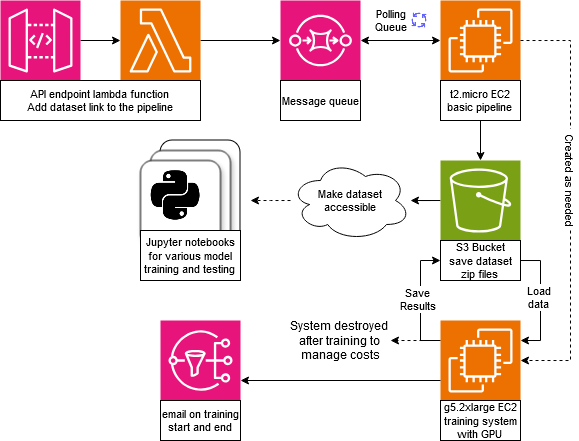
\includegraphics[width=0.5\linewidth]{images/AWS_diagram.png}
	\caption{Initial data cloud pipeline}
	\label{fig:aws-pipeline}
\end{figure}

\begin{figure}[!htb]
	\centering
	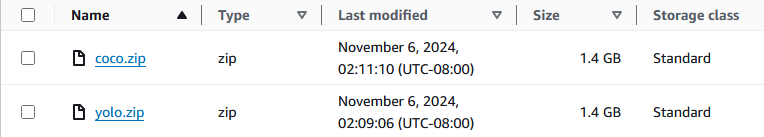
\includegraphics[width=0.75\linewidth]{images/s3_bucket.png}
	\caption{View of our S3 bucket}
	\label{fig:s3}
\end{figure}

\printbibliography

% \appendix

\end{document}
